% Foveated Vision on a Moving Head: Depth from Forward Motion
% VISGRAF Lab technical note. 15 November 2026.
% Build: pdflatex twice. Figures in figs/ come from the records of visgraf/foveal-motion (figs/SOURCES.md).
\documentclass[11pt,a4paper]{article}

\usepackage[T1]{fontenc}
\usepackage[utf8]{inputenc}
\IfFileExists{lmodern.sty}{\usepackage{lmodern}\usepackage{microtype}}{\usepackage[expansion=false]{microtype}}
\usepackage[a4paper,top=2.5cm,bottom=2.6cm,left=2.6cm,right=2.6cm]{geometry}
\usepackage{textcomp}
\usepackage{amsmath,amssymb}
\usepackage{booktabs}
\usepackage{tabularx}
\usepackage{array}
\usepackage{multirow}
\usepackage{xcolor}
\usepackage{enumitem}
\usepackage{graphicx}
\usepackage[font=small,labelfont=bf]{caption}
\usepackage{placeins}
\usepackage[hidelinks]{hyperref}
\hypersetup{colorlinks=true,linkcolor=black!70!blue,citecolor=black!70!blue,urlcolor=black!70!blue,
  pdftitle={Foveated Vision on a Moving Head: Depth from Forward Motion},
  pdfauthor={Luiz Velho, with Claude (Anthropic)},
  pdfsubject={VISGRAF technical note, 15 November 2026}}

% ---------------------------------------------------------------- VISGRAF cover
\IfFileExists{techrep-ic.sty}{%
  \usepackage{techrep-ic}%
  \newcommand{\MakeVisgrafCover}{%
    \TRNumber{16}   % <-- placeholder: set the report number (printed as TR-26-XX)
    \TRYear{26}
    \TRMonth{11}
    \TRAuthor{Luiz Velho, Claude}
    \TRTitle{Foveated Vision on a Moving Head:\\Depth from Forward Motion}
    \TRMakeCover}%
}{\newcommand{\MakeVisgrafCover}{}}

% ---------------------------------------------------------------- helpers
\newcommand{\code}[1]{\texttt{\small #1}}
\newcommand{\cell}{\raggedright\arraybackslash}
\newcolumntype{L}{>{\cell}X}
\newcolumntype{R}{>{\raggedleft\arraybackslash}X}
\setlist{itemsep=2pt,topsep=4pt}
\renewcommand{\arraystretch}{1.15}
\setlength{\emergencystretch}{1.5em}
\renewcommand{\topfraction}{0.9}\renewcommand{\bottomfraction}{0.6}\renewcommand{\textfraction}{0.08}\renewcommand{\floatpagefraction}{0.8}
% where a number comes from
\newcommand{\src}[1]{\textsuperscript{\,#1}}
\newcommand{\WS}{\src{W}}   % measured by Claude Code on the workstation
\newcommand{\SB}{\src{S}}   % measured in the Chat sandbox

\title{\textbf{Foveated Vision on a Moving Head:\\Depth from Forward Motion}}
\author{Luiz Velho\\[2pt] \normalsize with Claude (Anthropic)\\[2pt]
  \normalsize VISGRAF Lab, IMPA}
\date{\normalsize Technical Note \textperiodcentered{} 15 November 2026\\[2pt]
  \normalsize Software and records: \url{https://github.com/visgraf/foveal-motion}}

\begin{document}

\MakeVisgrafCover
\maketitle

\begin{abstract}
\noindent A foveated eye walks straight ahead, looking where it goes. Can it see depth from its own motion, using only
its images? Under a forward step every point moves along its radial line from the focus of expansion, and in the
log-polar coordinate $q=\ln\tan e$ it moves by $d=-\ln(1-t\zeta)$, the same for every eccentricity at a given inverse
depth~$\zeta$. We match that motion in two ways. M3 matches two frames: it is accurate where it accepts (held-out median
range error 0.9\,\% in a calibration room and 1.8\,\% in the Blender Classroom, with honest 95\,\% intervals), but it
covers too little of the field to pass the gates we declared beforehand (0.33 and 0.12 of the gated pixels, against 0.50
and 0.25). M4 matches a window of frames at once, summing every frame's cost along the common $\zeta$ axis (multiple-baseline
stereo moved to log-polar coordinates). With five frames on each side of the reference it passes both gates on held-out
frames: coverage 0.503 and 0.368, median error 0.42\,\% and 1.1\,\%, no error over 50\,\% in the Classroom. With five
frames behind only, it stays at M3's level. Frames behind and ahead of the reference close the matching cost's plateau
from opposite sides. What M4 still leaves is mostly depth edges, where a centred window cannot measure.
\end{abstract}

\noindent\small Numbers carry their source: \WS\ measured by Claude Code on the RTX~4090 workstation; \SB\ measured in
the Chat sandbox (2 CPU cores). Every number is in a record of the repository (\code{docs/motion.md} and
\code{docs/runs/issue-*/}) or in the GitHub issue that reported it.\normalsize

% ================================================================================================
\section{Why forward motion}\label{sec:why}

The first note of this series~\cite{tr1} moved the head for the first time: one foveated eye on the cyclopean point,
walking down the Blender Classroom. It found that looking along the path, the fovea gets no usable range: its finest
pixels sit at the focus of expansion (FOE), where there is no parallax. Fixating a point off the path, the fovea gets
range within a few per cent. That note matched pixels by an oracle: the renderer said which pixel of one look sees the
point of another.

This note drops the oracle. The eye looks straight ahead along a straight path (the dolly's \code{ahead} mode), the case
where the fovea gains least, and must find depth in the images themselves. Two things make the case attractive. Forward
motion is the most common motion of a walking observer. And it suits the foveated sensor's geometry: the flow is radial
from the FOE, the sensor samples densely around it, and in log-polar coordinates the flow becomes a shift along one
axis~\cite{schwartz,tistarelli}. The question is how much of the field gets a depth one can trust, and how good that
depth is.

% ================================================================================================
\section{Geometry}\label{sec:geometry}

Let $e$ be a ray's eccentricity from the heading and $\varphi$ its azimuth. A static point at range $\rho$ has axial depth
$z=\rho\cos e$; write $\zeta=1/z$. After a step $t$ along the heading its axial depth is $z-t$ and its lateral offset is
unchanged, so $\tan e' = \tan e\,z/(z-t)$ and $\varphi'=\varphi$. In the log-tangent coordinate $q=\ln\tan e$,
\begin{equation}\label{eq:d}
  d = q'-q = -\ln(1-t\zeta), \qquad t\zeta<1,
\end{equation}
with $t>0$ for a frame ahead of the reference and $t<0$ for a frame behind. Three consequences shape everything below.
\begin{enumerate}
\item \textbf{At a given depth the shift does not depend on where the point is.} A wall facing the eye moves as one
  rigid shift in $q$ (Figure~\ref{fig:geometry}a). Depth is a single number per point; the same unknown $\zeta$ explains
  every frame of a sequence, each with its own $t$.
\item \textbf{In pixels, the fovea sees almost no motion.} An angle step is $de = d\,\sin e\cos e$. The Foveated
  sensor's spacing grows as $s(e)=s_0(1+e/E_2)$~\cite{fovrendertr}, so a shift $d$ is $d\sin e\cos e/s(e)$ pixels:
  vanishing at the centre, then nearly flat across the periphery. The finest pixels see the smallest motion.
\item \textbf{Texture that is constant along radial lines cannot be matched,} with any number of frames: the motion is
  along those lines (the aperture problem, here exact).
\end{enumerate}
A matched displacement $d\pm\sigma_d$ gives $\zeta=-\operatorname{expm1}(-d)/t$ and $\sigma_\zeta=\sigma_d\,(1-t\zeta)/|t|$.
We call a range \emph{usable} when its 95\,\% interval is within $\pm10$\,\%.

\begin{figure}[t]
\centering
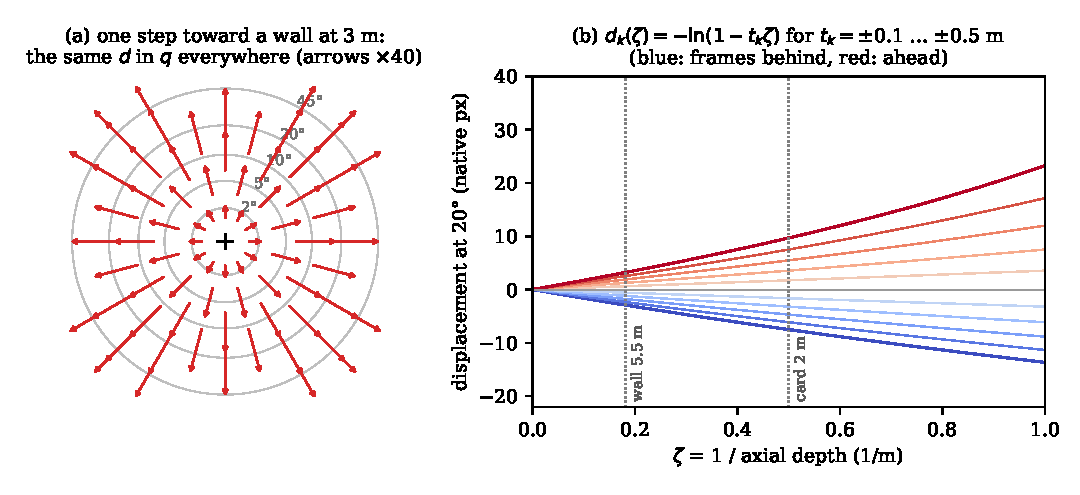
\includegraphics[width=\linewidth]{figs/geometry.pdf}
\caption{Forward-motion geometry on the foveated sensor. (a) One 0.099\,m step toward a wall at 3\,m: the same shift
$d=0.034$ in $q$ everywhere, drawn on the raster (radius $\propto E_2\ln(1+e/E_2)$, arrows magnified $\times40$); it is
shortest at the FOE. (b) The shift of each frame of a window of ten frames, $t_k=\pm0.1\ldots\pm0.5$\,m, in native pixels
at $20^\circ$: one unknown $\zeta$ explains all ten.}\label{fig:geometry}
\end{figure}

% ================================================================================================
\section{Setup}\label{sec:setup}

\textbf{Sensor.} fov-render's \code{Foveated} sensor~\cite{fovrender,fovrendertr}: a log-polar-like raster, fovea
$E_2=2^\circ$, field $e_{\max}=45^\circ$, profile \code{full} ($253\times253$ pixels). The eye is the cyclopean point
at 1.5--1.6\,m; head poses are known exactly.

\textbf{Scenes and paths.} Two scenes, each with a straight path at constant height, looking along it:
\begin{itemize}
\item a \emph{calibration room} from fov-render: a checkered room with about forty Siemens-star cards floating at about
  2\,m in front of walls at about 5.5\,m; 22 looks, 0.10\,m apart (Figure~\ref{fig:m3});
\item the \emph{Blender Classroom}: 47 looks, 0.099\,m apart, from the back of the room toward the board.
\end{itemize}

\textbf{Renders.} Blender Cycles through fov-render, OptiX on the workstation, at 1024 samples per pixel with an
independent seed per look (decision M-D12). M3 first ran at 64 samples with one seed: the noise was 20--30\,\% of the
signal and repeated across frames, and one Classroom pair kept 4\,\% of its anchors usable; at 1024 samples, 21\,\%\WS.
The noise of a render matters more than any matcher setting we tried.

\textbf{Anchors.} Every native pixel of the reference look between $1^\circ$ and $44^\circ$ eccentricity, about 48{,}750
per look.

% ================================================================================================
\section{How we evaluate}\label{sec:protocol}

The protocol is common to M3 and M4 and was declared before any measurement (issue \#5 of the repository).
\begin{enumerate}
\item \textbf{Truth-free estimation.} The estimator reads only images, poses and the sensor model. Truth (the renderer's
  Position pass) is read only by the evaluation.
\item \textbf{Calibrate one number.} The interval scale is the 95th percentile of $|\text{error}|/\sigma$ divided by
  1.96, over the interior anchors of a declared set of calibration-room frames. Nothing else is tuned on renders.
\item \textbf{Freeze.} Settings, scale and the estimates are hashed (sha256). The held-out frames are estimated after
  the freeze and evaluated once; the Classroom imports the calibration room's scale and opens no truth before.
\item \textbf{Gates} (issue \#5). On the textured, jointly visible, interior (more than 2\,px from an object boundary)
  anchors at $5$--$40^\circ$: the calibration-room gate asks median range error $\le5$\,\%, p90 $\le10$\,\% and
  \emph{coverage} (the share of those anchors that get a usable range) $\ge0.50$; the Classroom gate asks $\le10$\,\%,
  $\le25$\,\%, at most 5\,\% of errors over 50\,\%, and coverage $\ge0.25$.
\item \textbf{Every check ships a control that must fail}, and no threshold moves to make anything pass.
\item \textbf{Ceilings first.} An oracle ladder replaces the matcher by the true correspondence, exact, rounded to the
  pixel or with Gaussian noise of a given size, so each result can be read against what perfect or sloppy matching
  would give. Synthetic fixtures (planes, a corridor, a periodic wall, a radial-edge wall, an occluding board) come
  before real renders.
\end{enumerate}

% ================================================================================================
\section{M3: two frames}\label{sec:m3}

\textbf{Matcher.} Both looks are unwrapped onto a log-polar grid. A coarse search scans zero-mean NCC along each radial
line for the shift $d$; then a Gauss--Newton fit on the native raster refines the shift, a radial stretch and a gain and
offset per patch~\cite{lucaskanade}. Windows are $\pm3$ native pixels radially and $\pm1$ in azimuth. Anchors are rejected,
each with a recorded reason, for too little radial texture, low NCC, an ambiguous second peak, a range beyond the far
envelope, a failed fit, forward--backward disagreement, a disagreeing half window, no support from the neighbours, or a
depth edge in the neighbourhood. Settings were fixed on the fixtures and frozen (commit \code{7bb5e70}).

\begin{figure}[t]
\centering
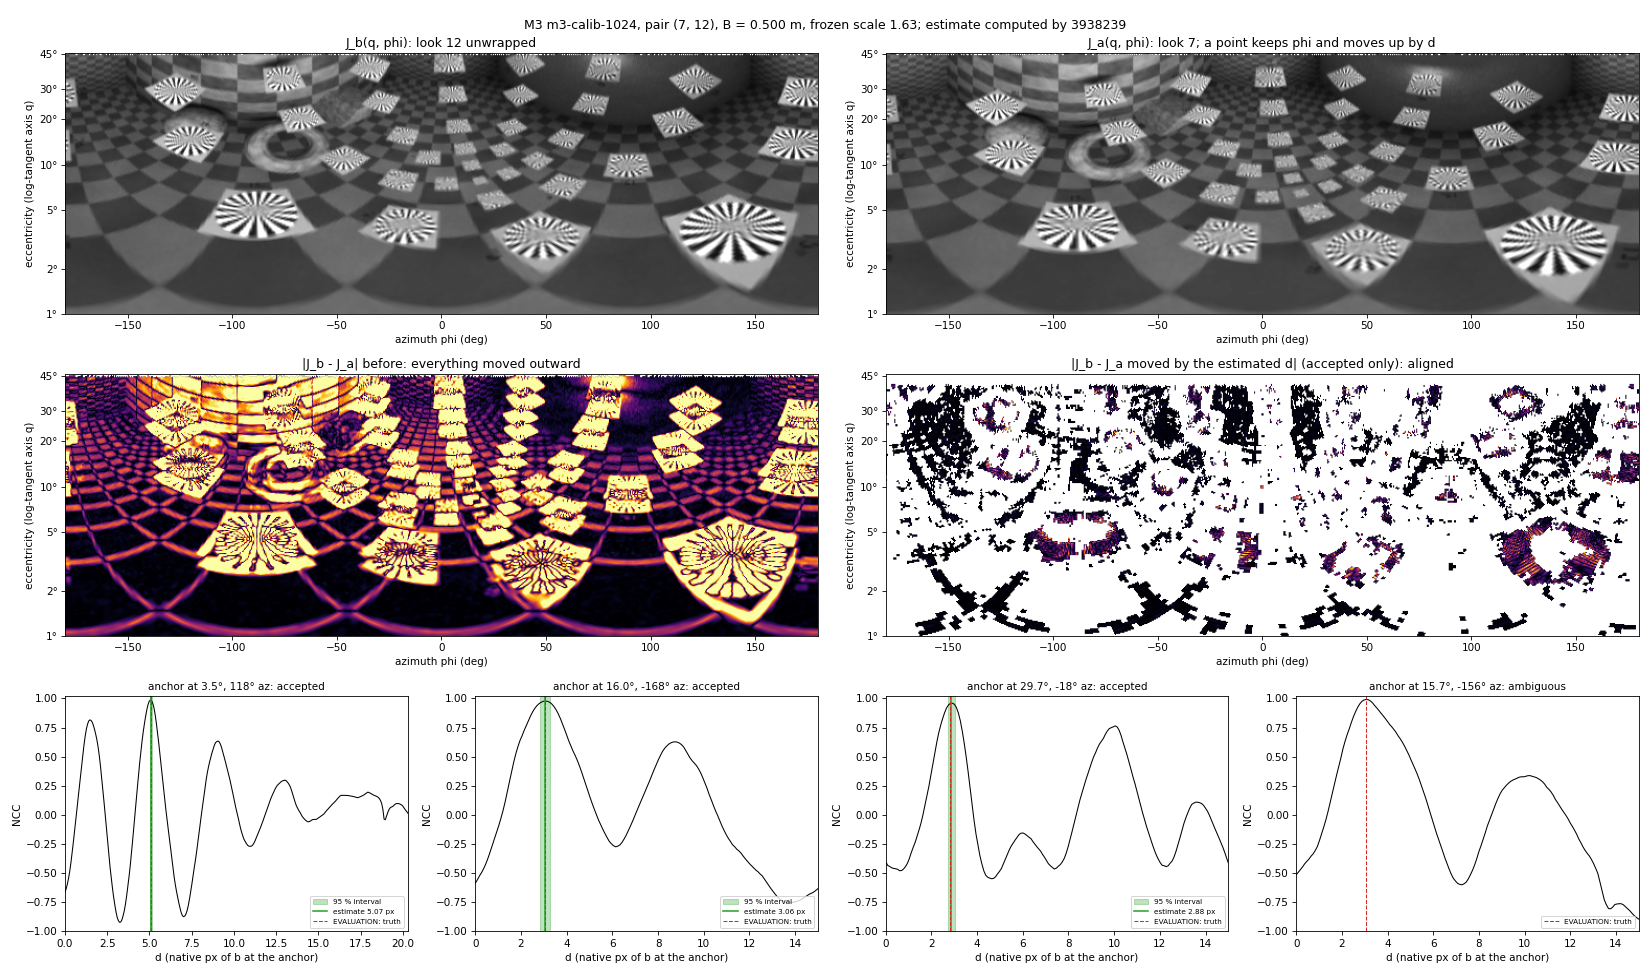
\includegraphics[width=\linewidth]{figs/m3_matching_calib_7_12.png}
\caption{M3 on the calibration room, pair (7, 12), 0.5\,m. Top: both looks unwrapped to $(q,\varphi)$; a point keeps its
azimuth and moves up. Middle: the difference before and after moving look~7 by the estimated $d$ (accepted anchors
only). Bottom: NCC along $d$ for four anchors; the last is rejected as ambiguous, with the truth (dashed) at its first
peak.\WS}\label{fig:m3}
\end{figure}

\textbf{Result} (Table~\ref{tab:m3}, held-out pairs 0.5\,m apart). Where M3 accepts, its depth is good: the median error
is 1--2\,\%, the intervals cover the truth 93--95\,\% of the time with the scale carried unchanged from one scene to the
other, and the accepted displacement error is 0.04--0.08\,px median. But only a ninth to a third of the gated pixels get a usable
range, and both gates fail on coverage alone. With true correspondences perturbed by 0.1\,px of noise, the same pairs
would make 0.83--0.87 of the field usable; M3 makes 0.20--0.24\WS. The losses are ambiguity (the stars' spokes, the checkers, the
chalk on the board), weak texture (walls, the board's interior) and the conservative edge tests. Over 1\,m, two frames do
worse than over 0.5\,m (stretch, occlusion and a long ambiguous search), as the fixtures predicted.

\begin{table}[h]
\centering\small
\caption{M3, held-out, 0.5\,m baseline (\code{docs/runs/issue-7/final/}; frozen \code{7bb5e70}, scale 1.625).}\label{tab:m3}
\begin{tabularx}{\linewidth}{@{}Lcc@{}}
\toprule
& calibration room (21 pairs) & Classroom (122 pairs) \\
\midrule
median / p90 range error & 0.9\,\% / 2.8\,\% & 1.8\,\% / 5.1\,\% \\
errors over 50\,\% & 0.3\,\% & 0.04\,\% \\
95\,\% intervals covering the truth (control: intervals $\times0.5$) & 0.949 (0.787) & 0.926 (0.712) \\
\textbf{coverage of the gated pixels} (required) & \textbf{0.332} ($\ge0.50$) & \textbf{0.116} ($\ge0.25$) \\
verdict & fail, on coverage & fail, on coverage \\
\bottomrule
\end{tabularx}
\par\smallskip\raggedright\footnotesize All measured\WS\ (Code at \code{3938239}).
\end{table}

% ================================================================================================
\section{M4: many frames}\label{sec:m4}

Equation~\eqref{eq:d} says that one unknown, $\zeta$, explains every frame of a sequence. M4 uses that directly. It is
Okutomi and Kanade's multiple-baseline stereo~\cite{okutomi}, moved from stereo disparity to the log-polar shift: each
frame's matching cost is put on the common $\zeta$ axis and the costs are averaged. The true minimum is shared by all
frames; the false minima of repeated texture fall at different $\zeta$ for different $t_k$ and wash out.

\textbf{Matcher.} \emph{Coarse}, on M3's log-polar grid: at a given $\zeta$ each frame's shift does not depend on the
eccentricity (consequence~1), so each frame's whole grid moves by one fractional row shift, and zero-mean NCC is averaged
over the frames whose window is valid, on a $\zeta$ grid of half a native pixel of the longest step, $\zeta=0$ included.
\emph{Fine}: one joint Gauss--Newton fit per anchor for $\zeta$, its radial slope $\partial\zeta/\partial q$ (which predicts
every frame's stretch consistently) and a gain and offset per frame, with $\sigma_\zeta$ from the joint covariance.
\emph{Frame consistency}: frames whose own NCC under the fit is below 0.5 are dropped and the fit repeated. M3's rejection
tests stay, plus too few frames ($<3$); the frames' mutual consistency replaces M3's forward--backward and half-window
tests. The matcher is written in PyTorch and runs unchanged on a CPU (the sandbox) and on CUDA (the workstation).

\textbf{Fixtures and controls}\SB. All 11 fixture gates pass. The periodic wall, M3's worst case, goes from 5\,\% accepted
(61\,\% of them wrong by more than a pixel) to 85\,\% accepted with none wrong; parallel corridor walls 1\,m away go from
15\,\% to 46\,\%. Three controls fail, as they must: shuffled frame steps, steps 20\,\% too long, and a \emph{foreign
geometry}. In that last control every window frame comes from the scene scaled 1.5$\times$ about the reference eye, with
its textures scaled too, so the reference image is unchanged to $10^{-14}$ while the frames see the wall at 4.5\,m instead
of 3\,m. The matcher accepts 93\,\% of the anchors, as on the true scene, and every depth is wrong (median 1.75\,px): no
image test can catch this; only the gate's truth does.

\textbf{Which window.} Table~\ref{tab:m4calib} compares three windows on the calibration room's held-out frames, each
calibrated and frozen separately, against M3 on the same pixels. Only the window with five frames on each side of the
reference passes. Five frames behind (the same longest baseline as M3's pair) does not beat M3. Ten frames behind, the
best window under the oracle (0.90 of the field usable at 0.25\,px per frame), falls furthest short with real images:
frames 1\,m back see the room too differently for its windows.

\begin{table}[h]
\centering\small
\caption{M4 on the calibration room, held-out frames, against M3's frozen matcher on the pair $(r-5,r)$ at the same
pixels (\code{docs/runs/issue-10/stage5/}).\SB}\label{tab:m4calib}
\begin{tabularx}{\linewidth}{@{}Lccccc@{}}
\toprule
window & scale & usable (field) & usable (fovea) & \textbf{gate coverage} & median / p90 \\
\midrule
M3 pair, 0.5\,m & 1.625 & 0.243 & 0.048 & 0.332 & 0.91\,\% / 2.80\,\% \\
M4, 5 frames behind & 1.650 & 0.222 & 0.032 & 0.351 & 0.87\,\% / 2.53\,\% \\
\textbf{M4, 5 frames each side} & 1.487 & \textbf{0.365} & \textbf{0.218} & \textbf{0.503} (pass) & 0.42\,\% / 1.81\,\% \\
M4, 10 frames behind & 2.094 & 0.179 & 0.039 & 0.292 & 0.50\,\% / 1.40\,\% \\
\bottomrule
\end{tabularx}
\par\smallskip\raggedright\footnotesize Held-out references $r=12$--20 (both sides: 12, 14, 16). Intervals cover the truth
0.947--0.955 throughout. The two-sided pass is narrow: 0.503 against 0.50, on three references.
\end{table}

\textbf{Why both sides.} Figure~\ref{fig:curves} shows each frame's NCC along $\zeta$ at four Classroom pixels. Where the
five frames behind leave a plateau, and the pixel is rejected as ambiguous, the frames behind lose correlation when
$\zeta$ is too large (the point taken too near), and the frames ahead lose it when $\zeta$ is too small. Their mean is
closed from both sides only when both are in the window. The same pixels' truth (dashed) sits at the closed peak.

\begin{figure}[t]
\centering
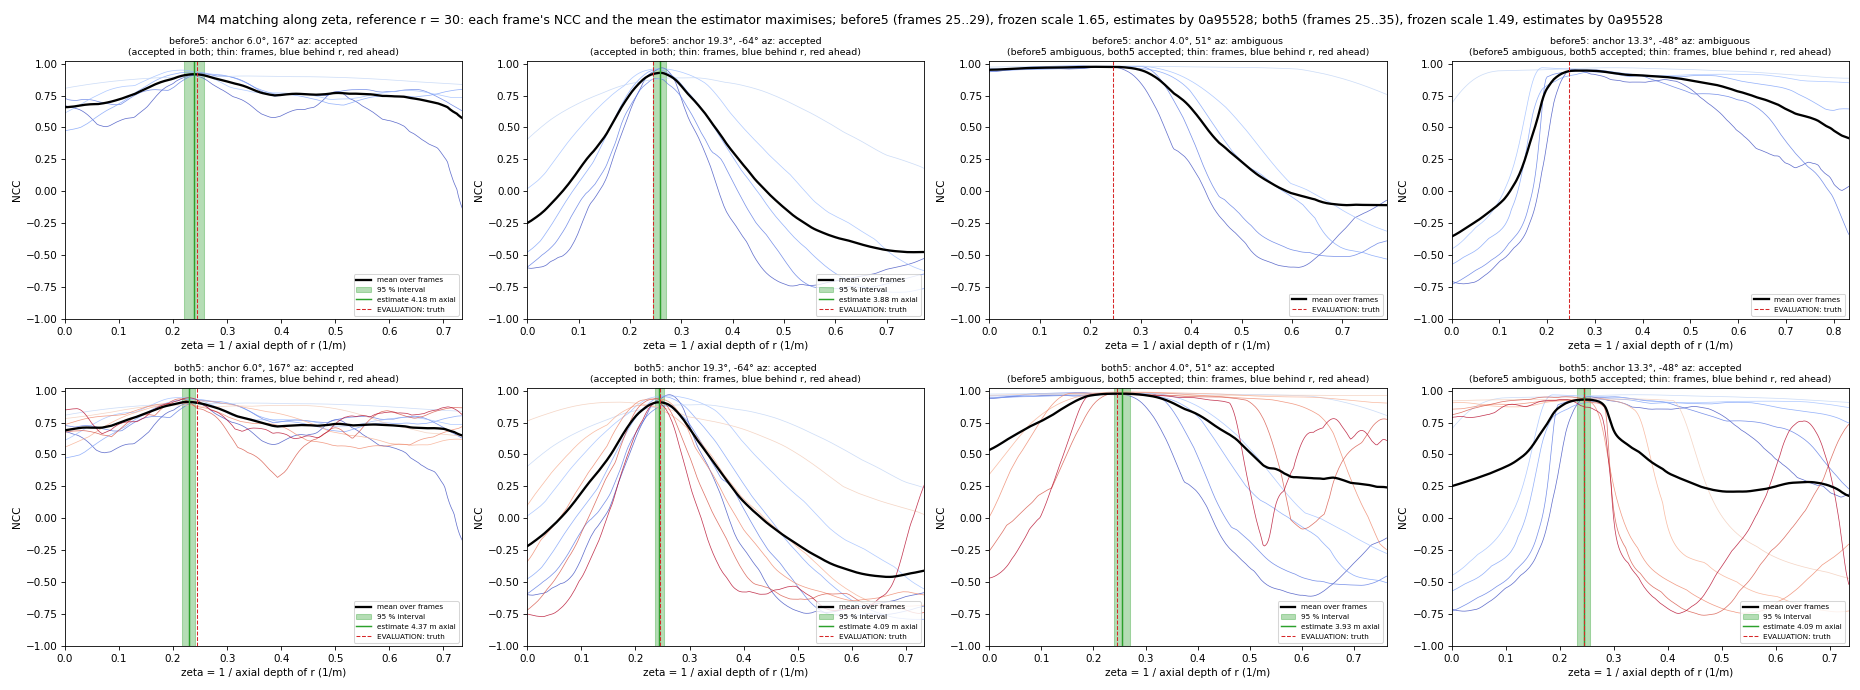
\includegraphics[width=\linewidth]{figs/m4_curves_classroom_r30.png}
\caption{M4 along $\zeta$ in the Classroom, reference $r=30$, at four pixels. Top row: five frames behind; bottom: five
frames each side. Thin lines: each frame's NCC (blue behind the reference, red ahead); thick: their mean, which the
estimator maximises; green: the estimate and its 95\,\% interval; dashed: the truth (evaluation only). In the two right
columns the window behind leaves a plateau; the frames ahead close it.\WS}\label{fig:curves}
\end{figure}

\textbf{The Classroom} (Table~\ref{tab:m4room}). The estimator and both scales were frozen on the calibration room
(\code{frozen.json}: the hashes of the estimator's files, the settings, the scales) and imported unchanged. Every
reference frame whose window fits was estimated: 33 with five frames each side, 37 with five behind, leaving out six
frames whose truth had been opened earlier. Before the Classroom, Code reran the calibration room on CUDA: scales,
counts and verdicts were identical to the sandbox's CPU run, with rates differing by at most $10^{-11}$\WS.

\begin{table}[h]
\centering\small
\caption{M4 on the Classroom, held-out, against M3's frozen matcher on the pair $(r-5,r)$ at the same pixels
(\code{docs/runs/issue-11/}; Code at \code{0a95528}).\WS}\label{tab:m4room}
\begin{tabularx}{\linewidth}{@{}Lcccc@{}}
\toprule
& \textbf{M4, 5 each side} & M3 pair & M4, 5 behind & M3 pair \\
\midrule
reference frames & 33 & & 37 & \\
\textbf{gate coverage} ($\ge0.25$) & \textbf{0.368} & 0.110 & 0.109 & 0.115 \\
median / p90 range error & 1.09\,\% / 3.51\,\% & 1.83\,\% / 5.24\,\% & 1.66\,\% / 4.65\,\% & 1.76\,\% / 5.09\,\% \\
errors over 50\,\% & 0 of 223{,}610 & 0.05\,\% & 0 of 76{,}197 & 0.04\,\% \\
verdict & \textbf{pass} & fail & fail & fail \\
usable: field / fovea & 0.455 / 0.255 & 0.196 / 0.050 & 0.212 / 0.038 & 0.202 / 0.064 \\
95\,\% intervals covering the truth & 0.939 & 0.920 & 0.917 & 0.921 \\
\bottomrule
\end{tabularx}
\par\smallskip\raggedright\footnotesize Controls, each failing: every step $\times1.2$ (median error 19.9\,\%);
intervals $\times0.5$ (coverage 0.748 and 0.663).
\end{table}

\begin{figure}[t]
\centering
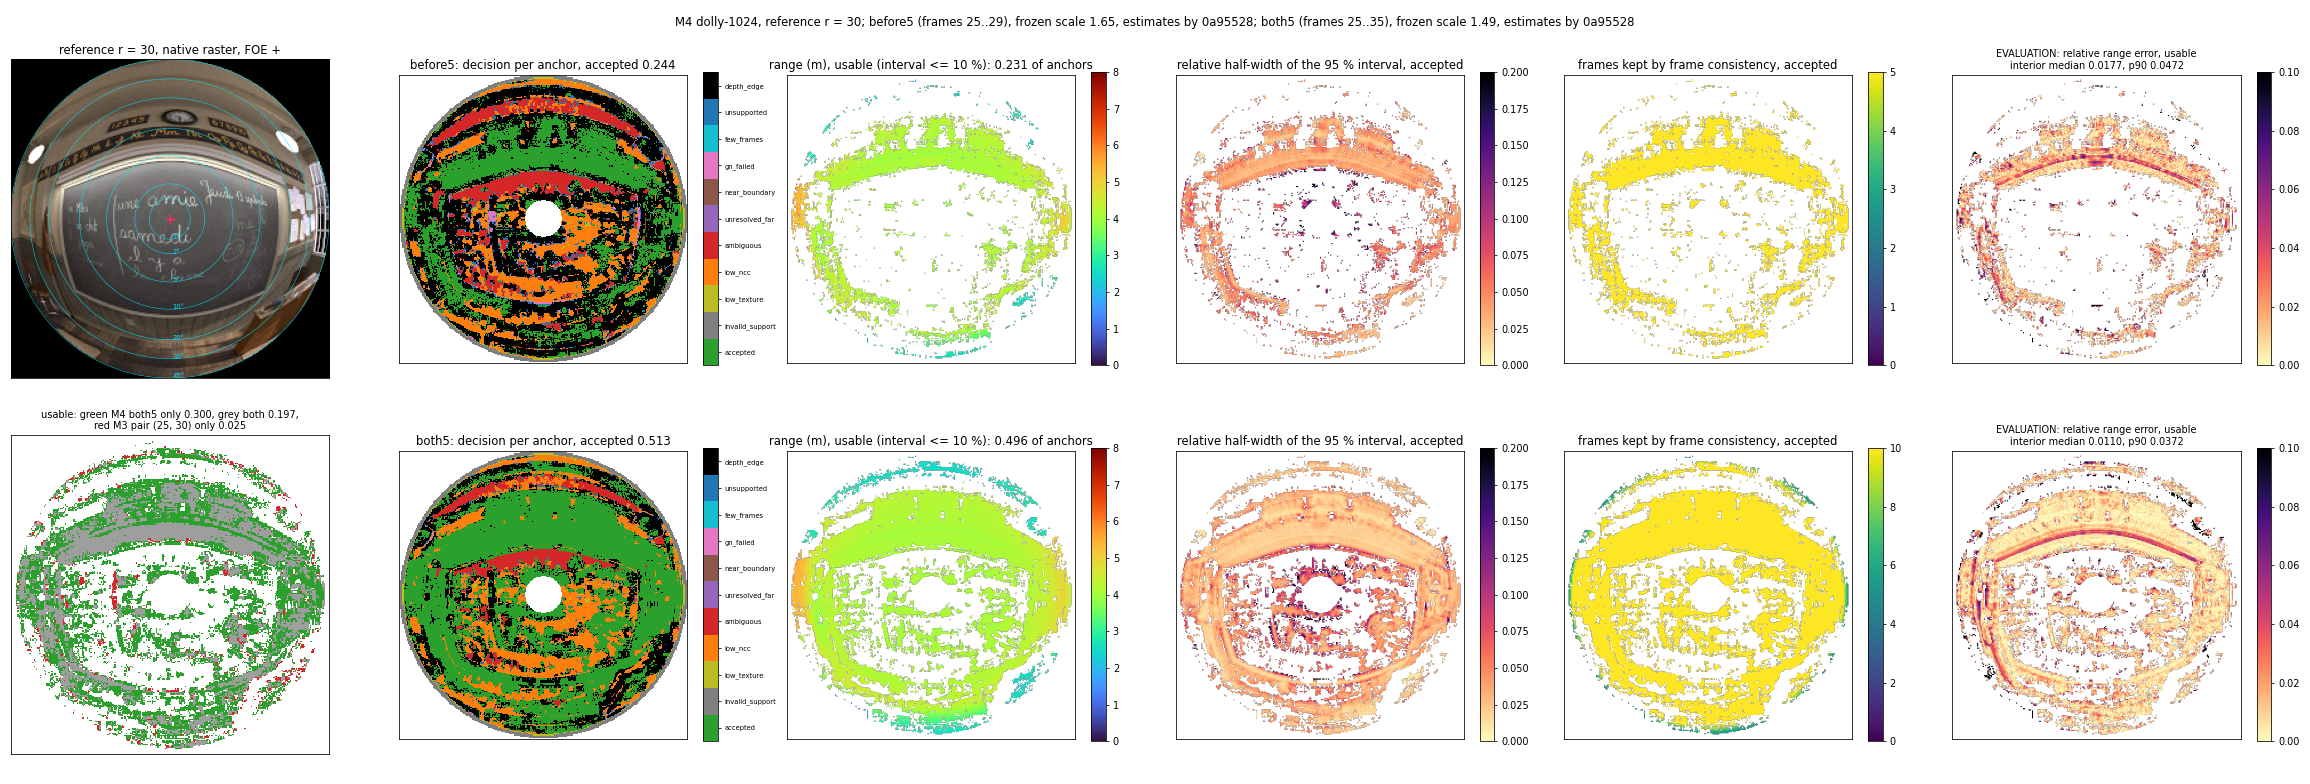
\includegraphics[width=\linewidth]{figs/m4_overview_classroom_r30.png}
\caption{M4 on the Classroom, $r=30$. Top row: five frames behind; bottom: five frames each side. From left: the
reference look (top) and which pixels are usable with M4 only (green), with both M4 and M3's pair (grey) or with M3 only
(red, 2.5\,\%); the decision per anchor; the range of usable anchors; the interval's relative half-width; the frames kept;
and the relative range error (evaluation only).\WS}\label{fig:overview}
\end{figure}

\begin{figure}[t]
\centering
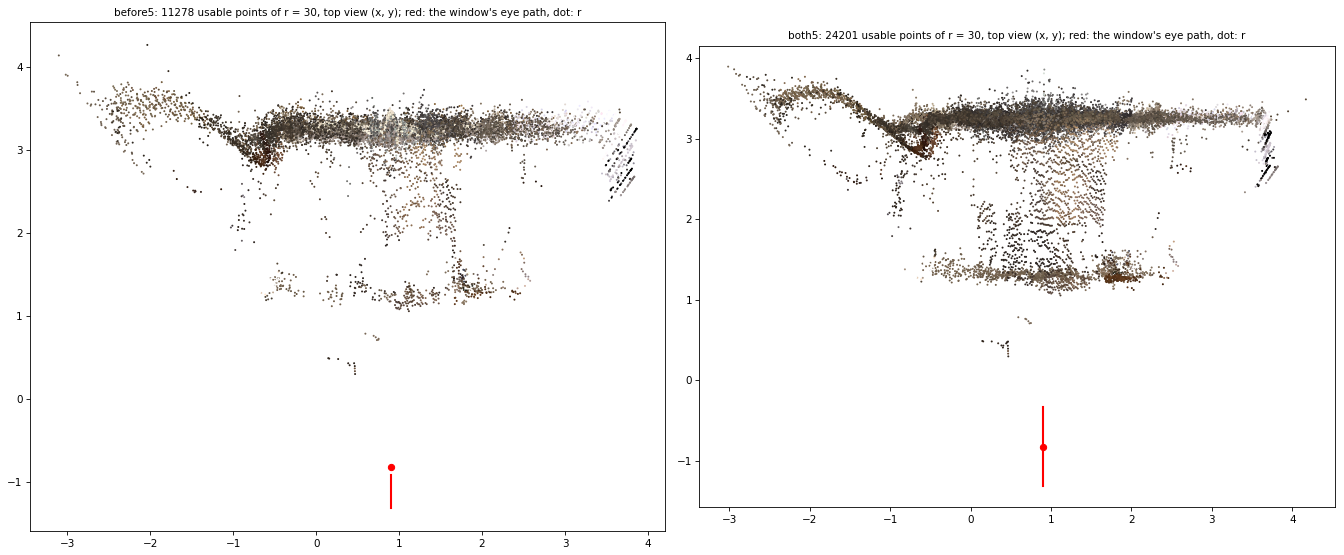
\includegraphics[width=0.78\linewidth]{figs/m4_cloud_classroom_r30.png}
\caption{The usable points of $r=30$ from above (metres; red: the window's eye path, dot: $r$). Left: five frames behind,
11{,}278 points; right: five each side, 24{,}201. The front wall with the board, and a band of surfaces at $y\approx1.3$\,m,
fill in with both sides; the streaks at the right are the window band of the side wall, M3's main error source too.\WS}\label{fig:cloud}
\end{figure}

With five frames each side, M4 more than triples M3's coverage of the gated pixels in the Classroom, at a lower error and
without gross errors, and it covers five times as much of the fovea (Figures~\ref{fig:overview} and \ref{fig:cloud}). From
one scene to the other its coverage drops from 0.50 to 0.37; M3's dropped from 0.33 to 0.12. The window behind only stays
at M3's level in both scenes: the frames ahead make the difference, at the cost of a five-frame delay (about 0.5\,m of
travel) before a frame's depth is known.

\textbf{Against the ceiling} (Table~\ref{tab:ladder}). With the exact correspondence both windows would make nearly the
whole field usable; the real matcher behaves like one whose correspondences are off by 0.25--0.5\,px per frame. The two-sided
window tolerates such a matcher far better.

\begin{table}[h]
\centering\small
\caption{Field usable in the Classroom: the oracle ladder at the same references, against the real matcher
(\code{docs/runs/issue-11/oracle.json}).\WS}\label{tab:ladder}
\begin{tabularx}{\linewidth}{@{}Lcccccc@{}}
\toprule
& exact & 0.05\,px & 0.1\,px & 0.25\,px & 0.5\,px & \textbf{RGB} \\
\midrule
M3 pair $(r-5,r)$ & 0.942 & 0.931 & 0.873 & 0.174 & 0.001 & 0.202 \\
M4, 5 behind & 0.994 & 0.987 & 0.964 & 0.540 & 0.046 & 0.212 \\
M4, 5 each side & 0.999 & 0.997 & 0.990 & 0.885 & 0.251 & \textbf{0.455} \\
\bottomrule
\end{tabularx}
\end{table}

% ================================================================================================
\FloatBarrier
\section{Where the remaining coverage goes}\label{sec:edges}

M4's largest remaining rejection is its depth-edge test: with five frames each side, about 30\,\% of the calibration
room's anchors\SB. The test predicts each neighbour in a $7\times7$ block from the anchor's $\zeta$ and radial slope and
rejects at a miss of 0.5\,px. Applying the same test to the true depth sorts the rejections by cause (calibration frames
only\SB): three quarters lie on real depth discontinuities, where a centred window straddles two surfaces and the depth
would be poor if accepted (39\,\% of them off by more than a pixel); a quarter are tripped by noisy neighbours and are mostly
measurable; none is caused by slope or curvature, even on a plane tilted $50^\circ$ (Figure~\ref{fig:edges}). Two lessons
follow. Pixels on an edge mix two surfaces across their footprint, so a one-ray truth is itself ill-defined there; on one
calibration frame, even M4's accepted pixels within 2\,px of a boundary are 23\,\% off by more than a pixel against it, which is why the gates
leave them out. And a window that slides to one side of the edge should recover much of what is lost: on one calibration
frame, side windows raised the interior pixels with a depth from 45\,\% to 60\,\%, with the median error nearly unchanged
(0.49\,\% to 0.59\,\%) but twice as many large errors\SB. That probe is preliminary and was not carried further (decision M-D18).

\begin{figure}[t]
\centering
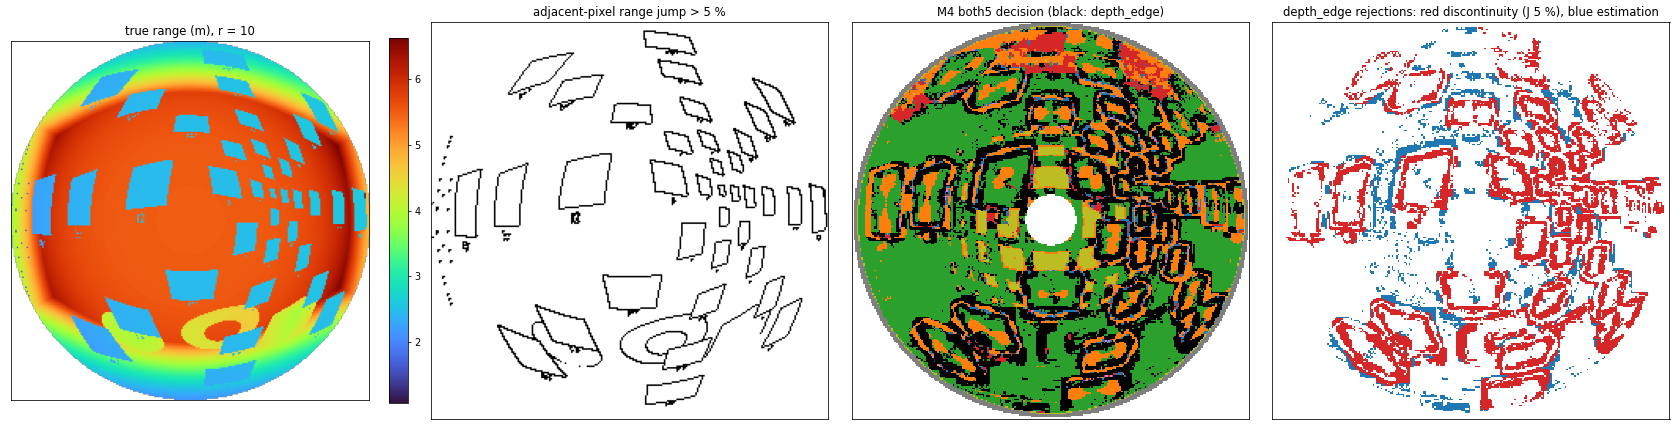
\includegraphics[width=\linewidth]{figs/m5_edges_calib_r10.png}
\caption{Depth edges in the calibration room, frame 10. From left: the true range; adjacent-pixel jumps over 5\,\%; M4's
decisions with five frames each side (black: rejected as a depth edge); and those rejections sorted by cause (red: a
real discontinuity in the $7\times7$ block; blue: tripped by noisy estimates).\SB}\label{fig:edges}
\end{figure}

% ================================================================================================
\section{How the work was done}\label{sec:process}

The method is the N-Surface method~\cite{nsurface} in the light form of the first note: one file of rules and GitHub
issues as the channel between Claude in a chat sandbox (``Chat''), which planned, wrote the code and its checks and ran
what two CPU cores can, and Claude Code on the RTX~4090 workstation (``Code''), which rendered, ran the Classroom and
reproduced the sandbox on CUDA. Luiz decided: ten recorded decisions (M-D9 to M-D18) over issues \#5 to \#16, among them
to freeze M3 and report its failure rather than tune it, to render again at 1024 samples, to choose the two-sided window
and accept its delay, and to stop the depth-edge work for this report. M3 and M4 took two days.

The protocol's refusals did much of the work. Three bugs in Chat's evaluation pipeline were caught because the pipeline
refused to go on, each before any held-out truth was read: a freeze that did not cover estimates appended after it, a
settings comparison that never matched, and a pose check that read a frame ahead of the reference as a $180^\circ$ heading
error. Smaller slips are disclosed in the records where they happened: a commit message that counted 16 checks instead of
11, a report that named the wrong commit, and a fixtures record that named the commit at the end of the run instead of
the code that ran. The CPU and CUDA results agree exactly, so the sandbox and the workstation could hand work to each other
without doubt about which machine produced a number.

% ================================================================================================
\section{Limitations}\label{sec:limits}

\begin{itemize}
\item \textbf{Synthetic images.} Rendered, noise-limited at 1024 samples per pixel, with no motion blur, rolling shutter
  or exposure changes; mostly textured, mostly matte surfaces. The Classroom's windows (transparency, reflections) hold
  most of the large errors.
\item \textbf{Known motion.} Head poses come from the path, not from the images: this is depth from known ego-motion.
\item \textbf{A non-causal window.} The passing window needs five frames after the reference; the causal one does not
  pass.
\item \textbf{The fovea stays the weakest part of the field,} as the geometry says it must: 22--26\,\% usable with the
  two-sided window, against 37--50\,\% coverage of the gated periphery.
\item \textbf{Two scenes, one path each,} and a narrow pass in the calibration room (0.503 against 0.50, on three
  references).
\end{itemize}

% ================================================================================================
\section{Next steps}\label{sec:next}

\begin{itemize}
\item \textbf{Side windows at depth edges}~\cite{kanadeokutomi,fusiello}, done properly: started on both sides of an
  edge, judged on all frames, and with depth edges as an output.
\item \textbf{Causal windows}: what a window that sees only the past can reach, for instance with longer windows of
  short steps or with a second eye.
\item \textbf{Estimated motion}: recover the step and the heading from the images before matching.
\item \textbf{The periphery in a gaze policy}: forward motion gives the periphery the depth and leaves the fovea little;
  that suggests looking off the path to put the fovea where parallax is.
\end{itemize}

\paragraph{Records.} Everything above is in \code{visgraf/foveal-motion}~\cite{fm}: \code{docs/motion.md} (decisions
M-D9 to M-D18 and all results), \code{docs/runs/issue-7/} (M3), \code{docs/runs/issue-10/} and \code{docs/runs/issue-11/}
(M4, with \code{frozen.json}), \code{docs/runs/issue-14/} on the branch \code{experiment/m5a-depth-edges} (the depth-edge
diagnosis), and issues \#5 to \#16. On the workstation the M4 matcher takes 2--3\,s per reference frame on CUDA, and the
whole Classroom evaluation 20\,min, most of it M3's comparison on the CPU\WS; in the sandbox, 65--110\,s per reference
frame\SB.

% ================================================================================================
\begin{thebibliography}{99}
\bibitem{fm} VISGRAF Lab. \emph{foveal-motion}: active foveal vision under head motion.
  \url{https://github.com/visgraf/foveal-motion}
\bibitem{tr1} Luiz Velho and Claude. ``Foveated Vision on a Moving Head: First Experiments''. VISGRAF technical note,
  12 November 2026. \url{https://github.com/lvelho/foveal-motion-tr}
\bibitem{fovrender} VISGRAF Lab. \emph{fov-render}: Blender Cycles rendering for gaze-directed binocular observers.
  \url{https://github.com/visgraf/fov-render}
\bibitem{fovrendertr} Luiz Velho and Claude. ``Foveated Stereo Rendering in Blender: A Unified Sensor Framework''.
  Technical Report TR-14-2026, VISGRAF Lab -- IMPA, 2026.
\bibitem{nsurface} Luiz Velho and Claude. ``The N-Surface Method: Rigor and Spontaneity in Human--AI Research''.
  VISGRAF technical note, 2026.
\bibitem{okutomi} M.~Okutomi and T.~Kanade. A multiple-baseline stereo. \emph{IEEE Transactions on Pattern Analysis and
  Machine Intelligence}, 15(4):353--363, 1993.
\bibitem{kanadeokutomi} T.~Kanade and M.~Okutomi. A stereo matching algorithm with an adaptive window: theory and
  experiment. \emph{IEEE Transactions on Pattern Analysis and Machine Intelligence}, 16(9):920--932, 1994.
\bibitem{fusiello} A.~Fusiello, V.~Roberto and E.~Trucco. Efficient stereo with multiple windowing. In \emph{Proceedings
  of the IEEE Conference on Computer Vision and Pattern Recognition}, pages 858--863, 1997.
\bibitem{lucaskanade} B.~D. Lucas and T.~Kanade. An iterative image registration technique with an application to stereo
  vision. In \emph{Proceedings of the 7th International Joint Conference on Artificial Intelligence}, pages 674--679, 1981.
\bibitem{schwartz} E.~L. Schwartz. Spatial mapping in the primate sensory projection: analytic structure and relevance
  to perception. \emph{Biological Cybernetics}, 25:181--194, 1977.
\bibitem{tistarelli} M.~Tistarelli and G.~Sandini. On the advantages of polar and log-polar mapping for direct estimation
  of time-to-impact from optical flow. \emph{IEEE Transactions on Pattern Analysis and Machine Intelligence},
  15(4):401--410, 1993.
\end{thebibliography}

\end{document}
